%----------------------------------------------------------------------------------------
%	PACKAGES AND DOCUMENT CONFIGURATIONS
%----------------------------------------------------------------------------------------
\documentclass[11pt]{article}
\usepackage{amsmath} % Required for some math elements
\usepackage{hyperref} 
\usepackage{xcolor}
\usepackage{lipsum} 
\usepackage{cite}
\usepackage{graphicx} % Required for the inclusion of images
\usepackage{algorithmic}
\usepackage{array}
\usepackage{bookmark}
\usepackage{listings}
\usepackage{amssymb}
\usepackage{enumitem}
\usepackage[margin=24mm]{geometry}
\usepackage[caption=false, font=footnotesize]{subfig}
\usepackage{multirow}
\usepackage[active,tightpage]{preview}

\renewcommand{\PreviewBorder}{1in}
\newcommand{\Newpage}{\end{preview}\begin{preview}}

\newlist{steps}{enumerate}{1}
\setlist[steps, 1]{label = Step \arabic*:}

\hypersetup{ %color attributes of citation, link, etc.
    colorlinks=true,
    linkcolor=blue,
    filecolor=gray,      
    urlcolor=blue,
    citecolor=blue,
}

\newcommand{\matlab}{\textsc{Matlab }} %very important and totally necessary addition

\newcommand\Item[1][]{%
  \ifx\relax#1\relax  \item \else \item[#1] \fi
  \abovedisplayskip=0pt\abovedisplayshortskip=0pt~\vspace*{-\baselineskip}}
  %----------------------------------------------------------------------------------------
%	DOCUMENT INFORMATION
%----------------------------------------------------------------------------------------
 
\title{ECEN303 : Analogue Electronics \\ Filter Lab Submission}
\author{Daniel Eisen : 300447549}
\date{\today}

\begin{document}
\begin{preview}
\maketitle
%----------------------------------------------------------------------------------------
%	DOCUMENT CONTENT
%----------------------------------------------------------------------------------------
\section*{Introduction}
An active filter is a type of analogue circuit, typically implemented with an Op-amp to improve the cost, performance, and predictability of the filter design.

An amplifier prevents the load impedance of the following stage from affecting the characteristics of the filter. With tuning of these characteristics being easily set using resistors and capacitors. 
\section{Filter Design}
By utilising the online tool \href{https://tools.analog.com/en/filterwizard/}{Filter Wizard} and knowledge of filter design, a 2nd Butterworth filter was designed. 

\fbox{
        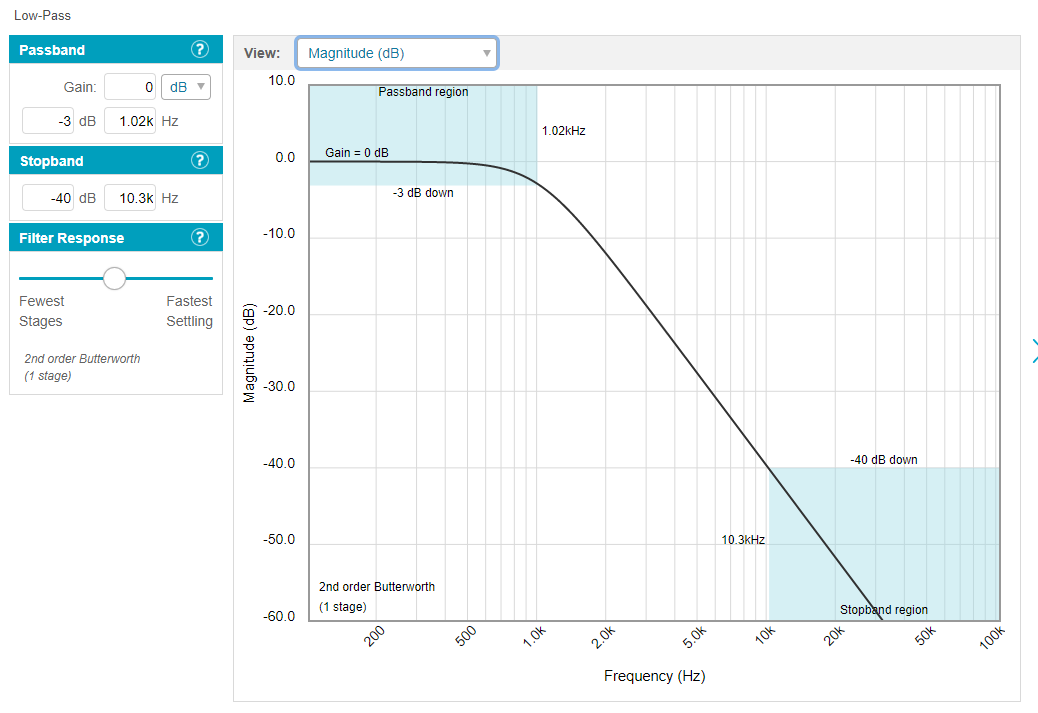
\includegraphics[width=0.5\textwidth]{images/wizard_design.png}
        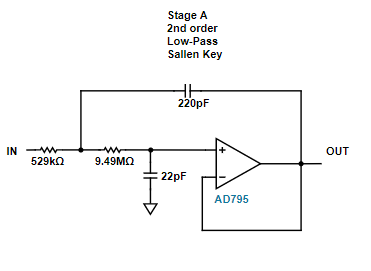
\includegraphics[width=0.5\textwidth]{images/wizard_circuit.png}
}
\begin{center}
        (a) \hspace*{0.2\textwidth} Figure 1. \hspace*{0.2\textwidth} (b)
\end{center}

Figure 1a shows the design specifications. With a passband of unity gain, a cut-off frequency ($f_c$) of 1023Hz. In order to restrain the filter to a second order the stop band had to be set at 10.2kHz at a minimum.

As this a Butterworth topology, it has the following characteristics:
$$K_c = 1, f_p = \frac{f_c}{K_c} Q = 0.707$$
$$\therefore f_p = f_c = 1023Hz$$

As a result the circuit (Figure 1b) was produced, utilising the AD795 and capacitor:resistor value ratio smaller the preserve gain falloff stability at higher frequencies.

\begin{center}
        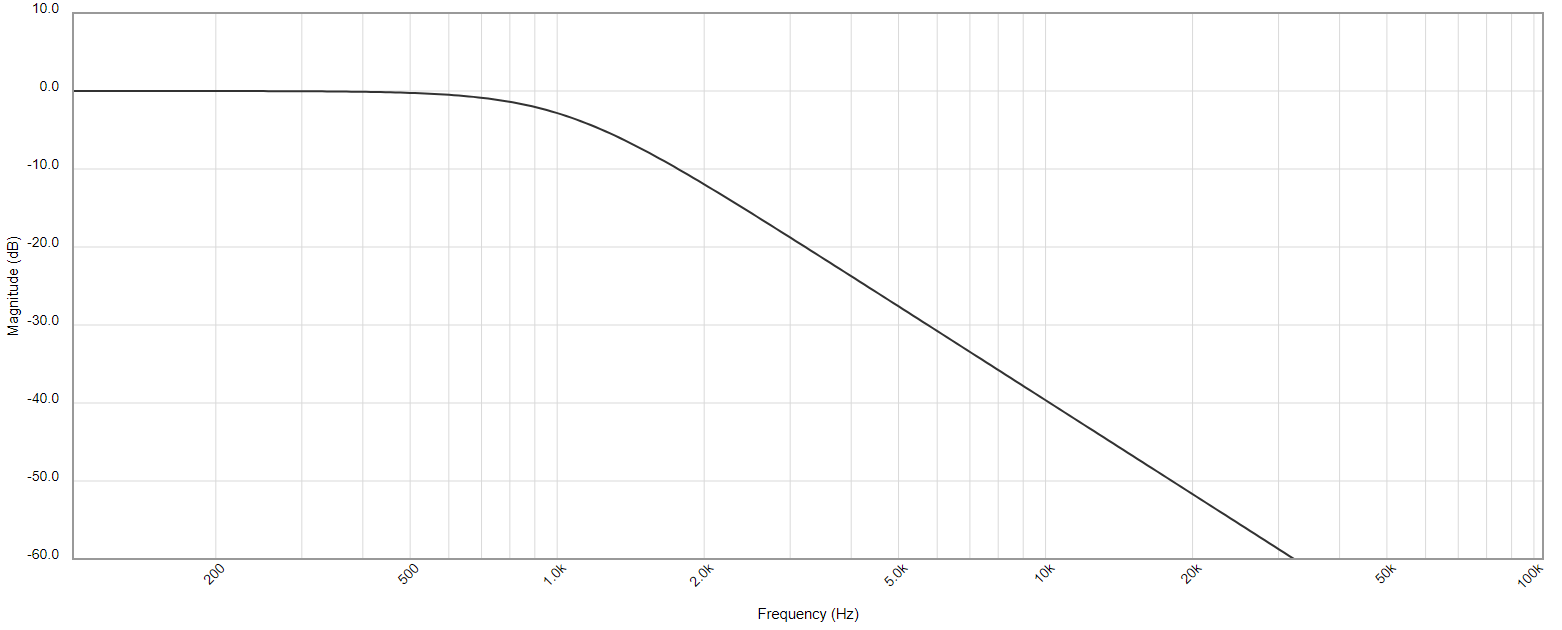
\includegraphics[width=0.6\textwidth]{images/wizard_mag.png}\\
        \vspace*{10mm}
        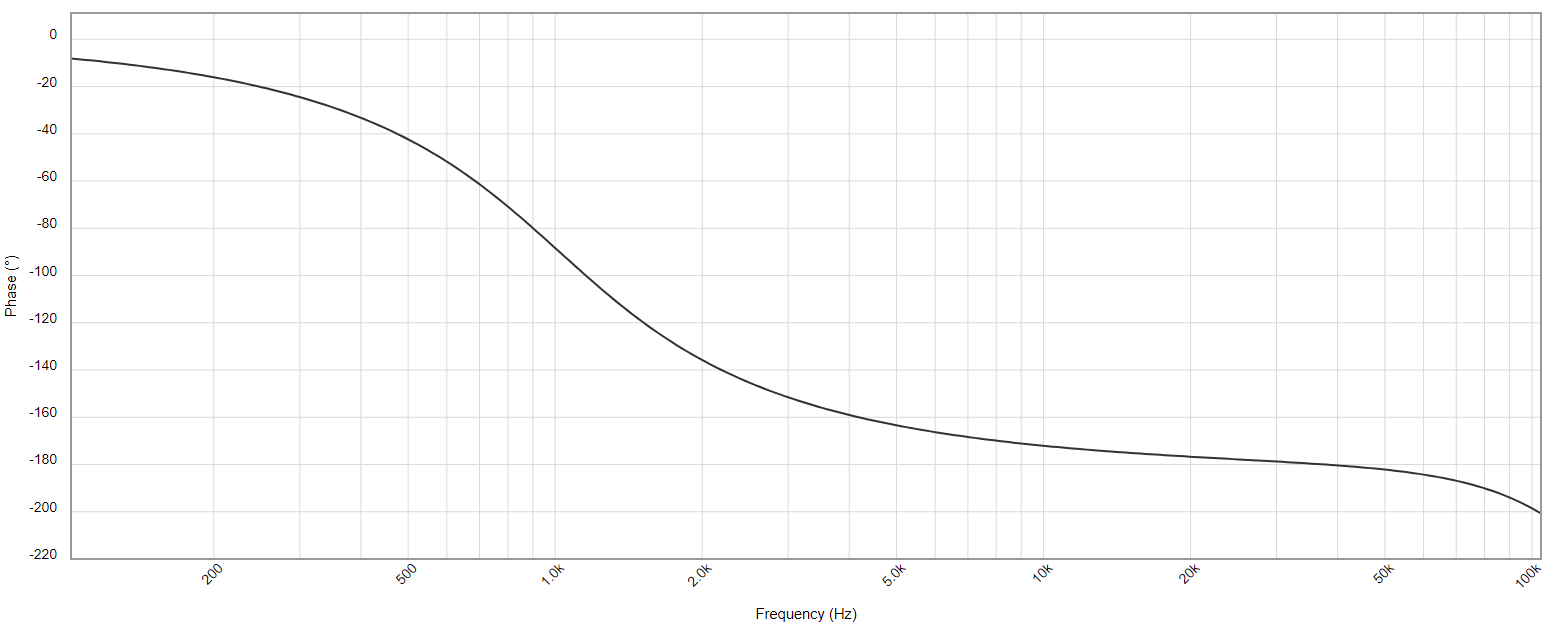
\includegraphics[width=0.6\textwidth]{images/wizard_phase.png}\\
        Figure 2.
\end{center}

Figure 2 shows filter wizards simulation of the filter frequency response, showing the poor phase integrity of the Butterworth topology. 


\section{Filter Simulation}
To confirm functionality and evaluation of the filter, it was reconstructed in LTspice and a AC frequency sweep analysis performed.

\fbox{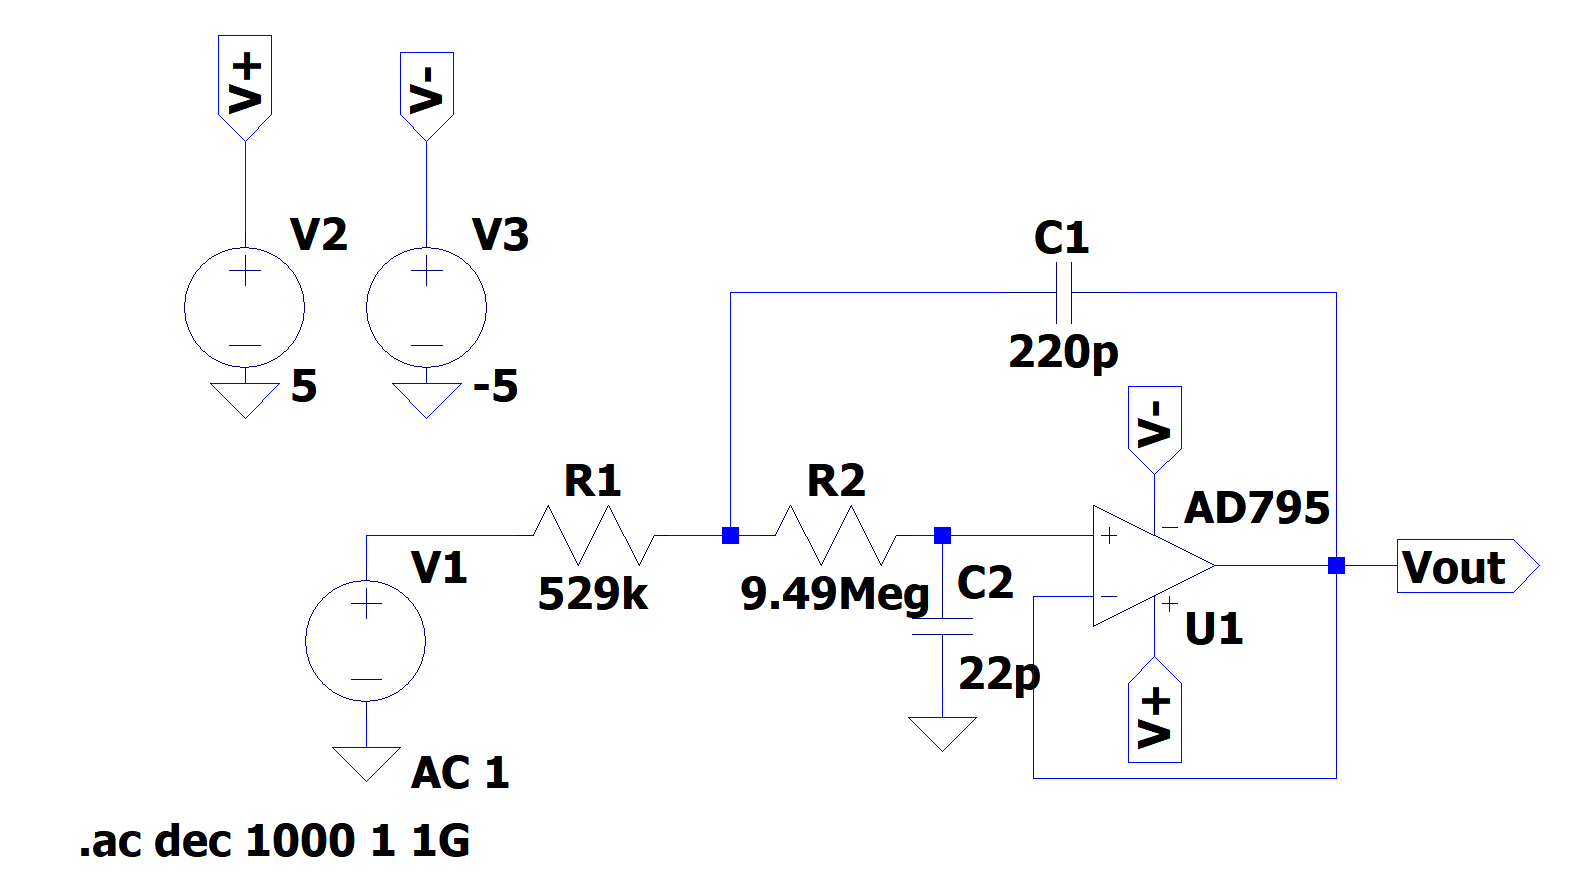
\includegraphics[width=0.45\textwidth]{images/spice_circuit.png}}
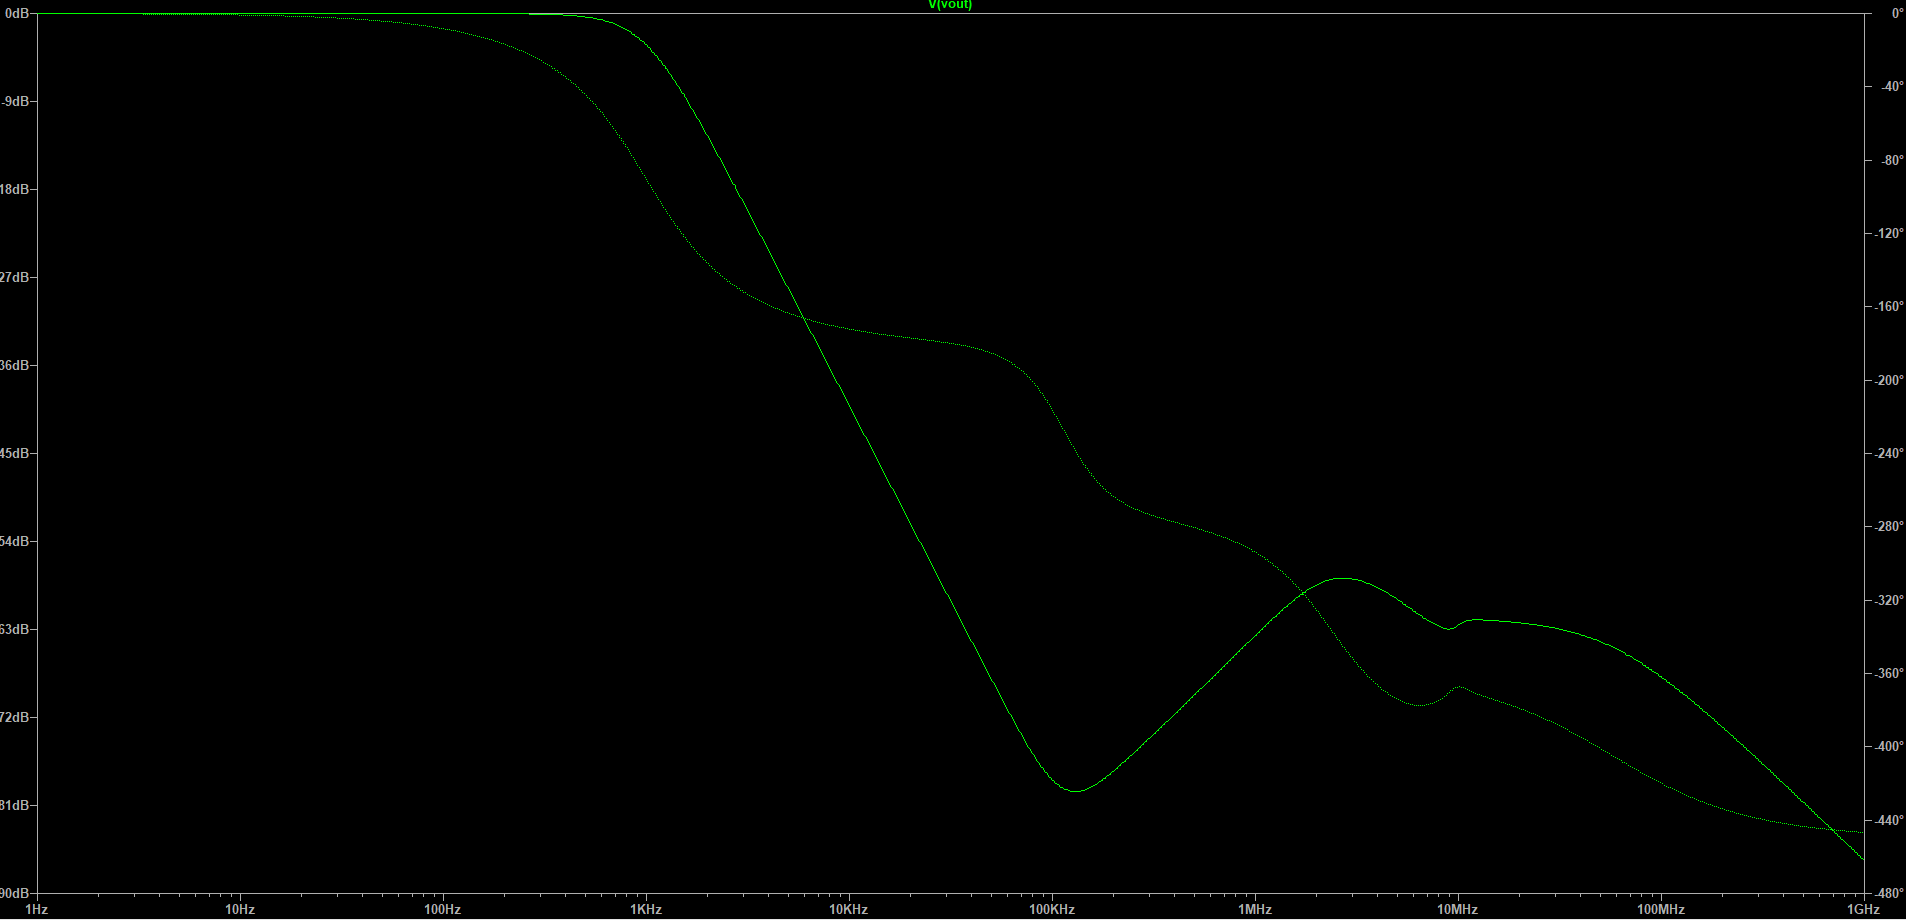
\includegraphics[width=0.55\textwidth]{images/spice_sim.png}
\begin{center}
        (a) \hspace*{0.2\textwidth} Figure 3. \hspace*{0.2\textwidth} (b)
\end{center}

Circuit reconstructed shown in Figure 3a. Simulation result shown in Figure 3b, extended to 1Ghz, confirming the phase integrity and gain falloff of the design.


\section*{Discussion}
\subsubsection*{Filter Topology}
There are many active filter approximations of the ideal 'Brick wall', all with their own drawbacks and advantages. 
In this case the Butterworth approximation was chosen. It has no pass-band ripple, that means, all pass-band frequencies have identical magnitude response but has bad selectivity, not really applicable for designs that require a small gap between pass-band and stop-band frequencies. This seen in our design requiring a band gap of ~9277Hz.


It was configured in the Sallen–Key topology, for simplicity of design and is a form of the VCVS design.
\subsubsection*{Sampling Frequency}
The minimum Sampling frequency to ensure no loss/distortion of signal is outlined by the Nyquist Theorem; the Nyquist critical frequency is 1 / (2 * sampling interval). You need at least two sampled points in every period that you want to capture. If there is significant information that you do not capture, you will have problems with aliasing and the signal integrity will be compromised.

\end{preview}
\end{document}